\appendix
\renewcommand{\thechapter}{}
\chapter{Paragrafi in italiano}
\renewcommand{\thechapter}{\Alph{chapter}}
%Necessario per rimuovere la lettera dall'appendice
\section{Joystick}
 Esistono due tipi di impugnatura per Joystick: Ball Top (sferica) e Bat Top (a goccia). I due usati per il cabinato sono a forma sferica, manufatti dall’azienda giapponese Sanwa. Il SANWA JLF-TP-8YT (Figura~\ref{fig:sanwaita}) è uno dei prodotti più popolari grazie alla sua precisione e sensibilità. Proprio per questo è il top di gamma per esperti di videogame picchiaduro, nei quali ogni centesimo di secondo conta. Di default, il joystick ha un Restrictor Gate che permette fino a otto movimenti. Essendo presenti solo quattro microswitch, le otto direzioni sono possibili grazie alla pressione contemporanea di due pulsanti.Il collegamento alla scheda di encoding è molto semplice e rapido grazie ad un un connettore a cinque fili (uno è la massa).\\
I componenti del joystick sono:\\
\textbf{Top}: L’impugnatura.\\
\textbf{Stick}: L’asticella del joystick.\\
\textbf{Disk}: Un dischetto di plastica utile per accompagnare la mano nei suoi movimenti. Oltre a coprire il buco nella plancia, ha anche una funzione estetica.\\
\textbf{Mounting Plate}: La piastra di metallo destinata al montaggio. Va fissata sotto la plancia tramite gli appositi fori con delle viti.\\
\textbf{Pivot}: Il pezzo che permette il movimento dell'asta della leva.\\
\textbf{Spring}: Una molla il cui scopo è far tornare in posizione neutrale (centrale) la leva. Tanto più la molla sarà larga, tanto più sarà la resistenza della leva negli spostamenti.\\
\textbf{Microswitch}: I piccoli interruttori su cui la Stick va a premere. Su questa specifica leva ce ne sono quattro.\\
\textbf{Restrictor Gate}: Il restrittore è un pezzo di plastica il cui compito è limitare i movimenti dell'asta.\\
\textbf{Actuator}: Uno spessore situato nella parte finale dello Stick. Dovrebbe incrementare la precisione della leva grazie ad una pressione più accurata sui microswitch.\\
\textbf{E-ring}: Il compressore della molla. Insieme alla Spring aiuta la leva a tornare in posizione neutra. Si chiama così perché la sua forma somiglia molto ad una “E”.\\
\begin{figure}[h!]
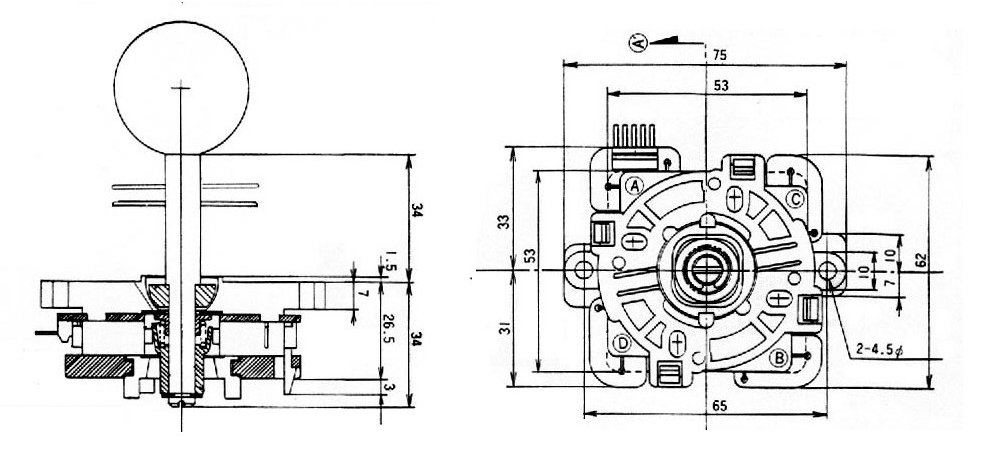
\includegraphics[scale=0.4]{joystick}
\centering
\caption{Sanwa JLF-TP-8YT (misure in mm)}
\label{fig:sanwaita}
\end{figure}
